\section{Methods}
\subsection{Preprocessing}
Each student of the 2016 class filled out several sheets of paper
with digits from 0 to 9. An example of this data
is shown in figure 
\ref{fig:handwriten_digits}. 
This section describes the preprocessing scheme
applied to this data before applying the machine learning algorithms.
\begin{figure}[h]
\centering
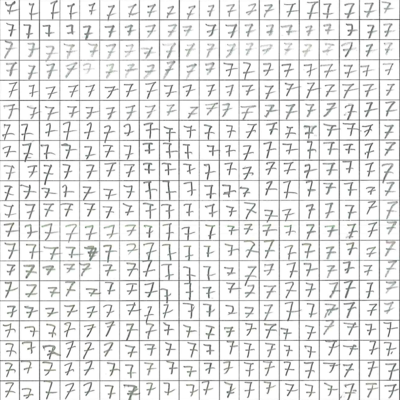
\includegraphics[width = 0.5\textwidth]{img/cropY2016G2M1-100-7.png}
\caption[Handwritten digits]
{
Handwritten digits. Scanned image. Cropped, rotated, scaled, stretched
and downsampled to 100 DPI.
}
\label{fig:handwriten_digits}
\end{figure}
Each of these sheets of paper was scanned by the student at a resolution of 300 DPI.

Each sheet held two 4x4" grids of 400 digits.
To ease the preprocessing task,
the student marked the pixel locations of the outer grid corners manually,
before submitting the dataset to the class database.

The datasets were of varying quality and format:
some images were color images while others were not,
most images were stretched and skewed to some degree,
and many digits were overlapping the grid.

As the corner locations were assumed to be known,
the images were rotated, stretched and scaled
by the perspective transform,
and then cropped,
to obtain ten images per student,
each being a 1200x1200 pixels image of 400 hand written digits.
This image was then downsampled to 200 DPI and to 100 DPI.
These preprocessing steps were done using MATLAB and ImageMagick.
After downsampling, the color images were converted to greyscale in R.

After color conversion, the images were smoothened in order
to make the digit data more uniform and easier to classify correctly.
It was chosen to apply a gaussian blur, as this smoothens
evenly in all directions.
The gaussian blur has one parameter named \(\sigma\),
and one which is the kernel size.
In this project, it was chosen to use the default
kernel size of \(2 \lceil3\sigma\rceil +1\),
and vary \(\sigma\) in order to find
optimal preprocessing parameters for the classification.

After smoothing the images of the grids,
each digit box (grid element) was extracted
as a vector of greyscale pixel intensities.
To avoid training the classifiers to recognize the parts
of the grid that are inside the digit boxes,
the digit boxes were cropped until the grid was no longer visible,
before vectorization.
A fixed cropping percentage of 10 \% along each border was used
(6 pixels border for 300 DPI, 4 pixels border for 200 DPI and 2 pixels border for 100 DPI).

Thus, at 300 DPI, a digit is represented in 2304 dimensions,
at 200 DPI, it is in 1024 dimensions,
and at 100 DPI, it is 256 dimensions.
Naturally, the computations involved in the classification
are faster when working with the lower-dimensional data.
As part of the \(\sigma\) optimization process,
it was therefore chosen to measure the k-NN classification
accuracy on the raw datasets at each pixel density,
giving an optimized \(\sigma\)-pixel density combination
for the digit recognition problem.

All above steps only need to be carried out once per
\(\sigma\)-pixel density combination.
The implemented R scripts thus compute this preprocessing
as an offline step, storing the preprocessed
datasets on disk.

\subsubsection{Principal Component Analysis}
In previous work, it was found that including Principal Component Analysis (PCA)
as a final step of the preprocessing could speed up the training
at an acceptable cost of reduced accuracy.

PCA is a statistical tool used for dimensionality reduction,
and works by creating new variables from the input variables.
These new variables, called principal components,
are linear combinations of the input variables,
and are ordered by how much of the input data variance they explain.
The statistical optimality of PCA is only achieved
when the input data is linear. This is not the case
for hand written digits. This may explain part
of the loss of accuracy.

As the main purpose of this project is the comparison of two algorithms,
it was chosen to apply PCA to the data before machine learning.
In addition, the PCA was used to verify the previous
steps of the preprocessing scheme qualitatively,
ensuring that the main data variance is not due to the grid lines of the input data.

The dimensionality reduction lies in transforming the input
data by a matrix representing the principal components
(the eigenvectors), and then using only the
first N components, enough to explain a given percentage of the cumulated variance.

The data transformation matrix obtained from one PCA
can be stored and applied to new data.
It was therefore chosen to include the PCA in the training of the classifiers,
storing the information necessary to transform new data
with the trained classifiers.
PCA is performed before training, on the training set,
and the number of components is chosen dynamically as the minimum
required to explain a given percentage of the cumulated variance
of the training set.
Thus, the tuning parameter investigated in this work,
is the percentage of the cumulated variance to explain,
making the PCA an online step of the preprocessing scheme.
The results of PCA are therefore not stored on disk,
except when saved along with trained classifiers.

\subsection{Datasets, resampling methods and classifier evaluation}
The datasets used in this project are described in this section,
along with the resampling schemes employed for reporting
overall classification accuracies.
The combination of dataset and resampling scheme makes
for the classifier evaluation schemes used in this project,
also described in this section.

All the data used in this project is contained in the dataset
denoted by \(D_{ALL}\), consisting of data from the 23
individuals who submitted their datasets.
Each of these individual datasets is denoted by the group number X
and group member index Y as \(GXMY\).
Ten individual datasets were selected from \(D_{ALL}\),
yielding a smaller dataset
\(D_{FEWER}=G1M1\cup G2M1\cup G3M1\cup G4M1\cup G5M1\cup G6M1\cup G7M1\cup G8M1\cup G11M1\cup G13M1\).

10-fold cross validation applied to a dataset containing data from more than
one individual is denoted the \textbf{MIX} method.
Here, data from each individual has a very high probability of
being represented in both the training set and the test set.

A method denoted by \textbf{LOO} was applied to datasets
containing data from \(n>1\) individuals by dividing
the data into \(n\) folds. Each fold contains data from \(n-1\)
individuals for training. The test data of each fold is the
data of the person not represented in the training set.

Four classifier evaluation schemes are defined:
\begin{itemize}
\item One Person:
Data from only one person is used,
and reported classification accuracy is found by 10-fold cross validation.
\item Single Persons:
One Person, applied to every persons dataset. The reported
classification accuracy is the mean of the 23 accuracies.
\item All Mixed:
\(D_{ALL}\), \textbf{MIX}.
\item All LOO:
\(D_{ALL}\), \textbf{LOO}.
\end{itemize}
The three schemes Single Persons, All Mixed and All LOO
were used for classifier comparison,
while One Person was used during preprocessing
scheme development.

\subsection{k-Nearest Neighbours}
k-Nearest Neighbours (k-NN)
is a supervised learning algorithm.
The method is non-parametric,
meaning that it does not make any assumption about the distribution of the input data.
The method is referred to as a lazy learning algorithm,
as it does not use the training data to do any generalization (abstraction).
Figure \ref{fig:knn-example} \citep{knnwiki} shows the basic principle of the algorithm.
\begin{figure}[h]
\centering
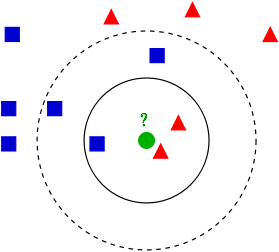
\includegraphics[width = 0.3\textwidth]{img/kNN-classification.png}
\caption[k-NN classification example]{
k-NN classification example, 2-dimensional 2-class data.
The test sample, the green circle,
has to be classified as one of the two classes indicated
as red triangles and blue squares, based on the number
of training samples close to the test samples.
With k=3 (the inner circle), the sample would be classified as belonging
to the class of the red triangles.
With k=5 (the outer dashed circle), the sample would be classified as belonging
to the class of the blue squares.
Author: Antti Ajanki \citep{knnwiki}.
}
\label{fig:knn-example}
\end{figure}

The purpose of the algorithm is to classify a
new \(n\)-dimensional test sample based on its \(n\) attributes
and the training samples that have been used.
The algorithm decides which class a new sample belongs to by
inspecting the k nearest neighbours,
and based on the class which is represented most strongly in the vicinity
of the test sample,
the class of the new sample is determined.
k can be both an even or an odd number.
In the case of a tie with a even numbered k,
the class of the test sample is randomly chosen among the classes holding
the majority of the votes.

The k-NN classifier performs differently with different k,
meaning k is a tuning parameter which can be used to optimize the classifier
to certain data.

Several metrics for measuring the distance between
two samples \(\mathbf{w}\) and \(\mathbf{v}\) can be employed,
including Euclidean distance, eq. \eqref{eq:euclidean-distance},
and Manhattan distance, eq. \eqref{eq:manhattan-distance}.
\begin{equation}
d(\mathbf{w},\mathbf{v}) = \sqrt{\sum_{i=1}^n (w_i - v_i)^2}
\label{eq:euclidean-distance}
\end{equation}
\begin{equation}
d(\mathbf{w},\mathbf{v}) = \sum_{i=1}^n \left|w_i - v_i\right|
\label{eq:manhattan-distance}
\end{equation}

The advantage of using k-NN is that it is simple to use,
and works well on basic problems.
However, it can be slow for real-time prediction applications,
especially if the dataset used for training is large,
as the method is a lazy learner.
Another disadvantage of the method is that it does not
learn anything from the training data, but just stores it;
No particular new insight is gained.
 
\subsection{Support Vector Machines}
Support Vector Machines (SVM) is a supervised learning
method that analyzes training data 
and tries to recognize patterns within the classification domain.
The standard SVM method is a binary classifier,
which predicts which of the two classes a given input belongs two. 
Prediction is done based on the model built from the training session.
The model provides a constraining border which makes the distinction
between the two classes.
The following introduction to SVM is based on \citep{svmwiki} and \citep{mlwr}.

For \(n\)-dimensional data,
SVM constructs an \(n\)-dimensional hyperplane or a set of hyperplanes.
The hyperplane with the largest distance to the nearest training sample
of any class (so-called functional margin), provides the best separation,
since it results in the clearest distinction between the classes,
and lower general error,
as illustrated by figure \ref{fig::SVM-illustrated} \citep{svmmathworks}.

The goal in SVM is to find this hyperplane which provides the optimal separation 
of the classes by having the widest margin. 

\begin{figure}[h]
\centering
%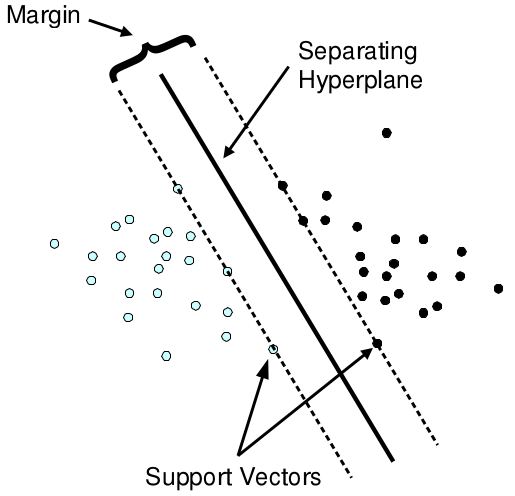
\includegraphics[width = 0.5\textwidth]{img/SVM-illu.png} %no source, Kiddi!
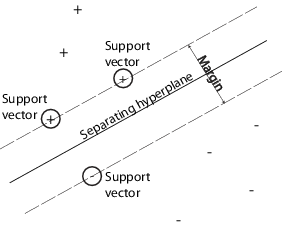
\includegraphics[width = 0.5\textwidth]{img/svmhyperplane}
\caption[SVM Illustrated]{SVM Illustrated. Source: \citep{svmmathworks}.}
\label{fig::SVM-illustrated}
\end{figure}

The training data for this method consists of a set of input vectors denoted as 
$\mathbf{x_i}$.
Each input vector has a number of component features. Each input 
vector is given a label, indicating its class.

The hyperplane is given by eq. \eqref{eq:hyperplane}.
\begin{equation}
\mathbf{w} \cdot \mathbf{x} + b = 0
\label{eq:hyperplane}
\end{equation}
$\mathbf{w}$ determines the orientation of the plane, and 
$\mathbf{b}$ is the offset of the plane from the origin.
 
The seperaing hyperplane which maximizes the margin can be found by examining 
the convex hull of each class’s training data and then find the closest points 
in the two convex hulls. The convex hull of a set of points is the
smallest convex set containing the points. If the hyperplane that bisects both 
convex hulls can be found, the resulting classifier is robust with
respect to the training data.
This concept is illustrated in figure \ref{fig:convex_hull} \citep{convexhull}.
\begin{figure}[h]
\centering
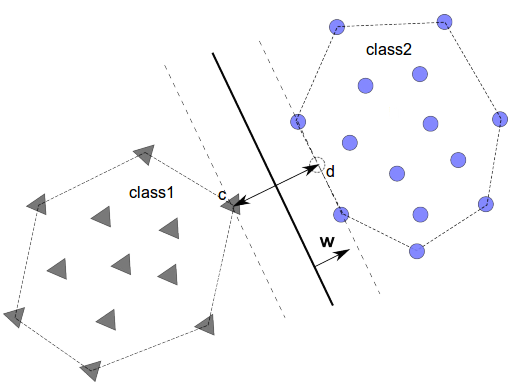
\includegraphics[width = 0.5\textwidth]{img/convex_hull.png}
\caption[Best plane bisects closest points in the convex hulls]
{Best plane bisects closest points in the convex hulls. The convex hulls 
are labeled c and d. Source: \citep{convexhull}.}
\label{fig:convex_hull}
\end{figure}  

To find the plane, the algorithm has to find the points closest
to the plane, which can 
be found by solving the quadratic programming problem of eq. \eqref{eq:quadratic-svm}.
\begin{equation}
min_\alpha~\left(\frac{1}{2} ||c-d||^2\right)
\label{eq:quadratic-svm}
\end{equation}
c and d are the closest to be found points,
defined by eqs. \eqref{eq:svm-c} and \eqref{eq:svm-d}.
\begin{equation}
\begin{aligned}
&c = \sum_{y_i~\in~class1} \alpha_ix_i  
& \text{subject to}
&& \sum_{y_i~\in~class1}\alpha_i =1 
&& \alpha_i \geq 0
\end{aligned}
\label{eq:svm-c} 
\end{equation}
\begin{equation}
\begin{aligned}
&d = \sum_{y_i~\in~class2} \alpha_ix_i  
& \text{subject to}
&& \sum_{y_i~\in~class2}\alpha_i =1 
&& \alpha_i \geq 0
\end{aligned} 
\label{eq:svm-d} 
\end{equation}
%Direct plagiarism:
%An alternative approach involves a search through the space of every possible 
%hyperplane in order to find a set of two parallel planes that divide the points 
%into homogeneous groups yet themselves are as far apart as possible.\\

In the case of non-linearly separable data,
a linear hyperplane cannot be used 
to define the solution. 
For this purpose is a slack variable introduced, which allows some points on the 
incorrect side of the margin, creating a soft margin, when a linear hyperplane 
was used to separate them.\\

A different approach for solving this problem would be using the kernel trick. 
The kernel trick involves transforming in $\mathbb{R}^n \rightarrow 
\mathbb{R}^{n+1}$. 
The challenging part is to find such transformation, $\phi$ which allow 
transforming data into a higher dimension in which it is separable. 

Kernel functions are in general in the following form:
\begin{equation}
K(\overrightarrow{x_i},\overrightarrow{x_j}) = \phi(\overrightarrow{x_i}) \cdot 
\phi(\overrightarrow{x_j}) 
\end{equation}

$x_i$ and $x_j$ illustrates two different feature vectors.

Previous work with the caret package of R
involved experimenting with the linear kernel of eq. \eqref{eq:linearkernel}
and the polynomial kernel of eq. \eqref{eq:polynomialkernel}
and showed promising results.
In particular, the polynomial kernel with a degree \(d=2\)
and a scaling factor \(s=0.1\) was found to yield generally good results.
\begin{equation}
K(\overrightarrow{x_i},\overrightarrow{x_j}) = (\overrightarrow{x_i}) \cdot 
(\overrightarrow{x_j})
\label{eq:linearkernel} 
\end{equation}
\begin{equation}
K(\overrightarrow{x_i},\overrightarrow{x_j}) = (s(\overrightarrow{x_i}) \cdot 
(\overrightarrow{x_j})+c)^d
\label{eq:polynomialkernel}
\end{equation}

The SVM algorithm used in this project is parametrized
by the cost of constraints violation \(C\),
a tuning parameter which is varied and chosen
according to classification accuracy.

\subsection{Parameter optimization}
The k-NN and SVM classifiers were each trained on the \(D_{FEWER}\) dataset with the \textbf{LOO} method.

\subsection{Parameter optimization on a smaller dataset}
To extract the most optimal parameter for training purposes was it decided, optimize the parameter on a smaller set consisting of 10 people data.  This was choosen, as it was desired gain the most optimal values for the varied dataset, such that the parameter found would be fit for a specific scenario, but a broad case. 
\todo[inline]{might have to be adjusted..}

\subsection{Test with data from single person}
\label{sec::test_with_data_from_single_person}

The first training were conducted with every single persons training set. The 
training using kNN consisted of k = 5,with a 10 - fold cross validation. k = 5 
was chosen, as it was shown from the parameter optimization that it would provide the highest accuracy on a varied dataset. \\

The training using SVM were performed using a polynomial kernel, with a degree 
of 2, scale of 0.1   and cost of 0.5 with a 10 fold cross validation as well. 
The polynomial kernel was chosen due to prior experiments with other kernel, and 
had a higher degree of freedom would provide a better accuracy. The parameter chosen was also found from the parameter optimization section. 
\todo[inline]{maybe a bit fluffy idk?}

 
A
10-fold cross validation uses 1 fold for testing and the rest for training 
purposes it thereby provides an average of the accuracies on how well a trained 
classifier, trained using the persons own data is capable of detecting himself.  
This information provides some insight on how consistent the persons writing is. 
An inconsistent writing style will cause lower mean accuracy compared to a 
consistent style. \\

Each accuracy is given an error bar stating the standard deviation of the 
dataset. The standard deviation of the mean accuracy is found by adding the 
internal standard deviation and the external standard deviation. The internal 
standard deviation is a vector of all individual standard deviation acquired 
from the 10-fold cross validation, an the external consist of the variance 
between the accuracies acquired  from the 10-fold cross validation. \\
 
The result of this test can be seen in section  \ref{sec::result}. 

\subsection{Test with data from all persons with a training set that includes 
data from all}

The dataset used for training here consist all the data mixed together. A 10-fold crossfold validation was also applied on to it from which an accuracy was computed. 



\subsection{Test with data from all persons where the training set does not 
include data from 
the persons in the test set}

The dataset consist of all the person, where the test was performed by leaving one out. A 10-fold crossfold validation was also applied onto it from which an accuracy was computed. 





